\subsection{Implementation}
\label{section:implementation}
The tug-of-war game was implemented in Unity3D and integrated with VR through SteamVR. Auditory feedback was provided for the countdown before the rope-pulling in order to increase the appearance of a gaming situation. Sounds were provided from the laptop speakers which was located behind the black curtains. To give users a sense of depth and maintain performance, we use mixed lighting methods\footnote{https://docs.unity3d.com/Manual/LightMode-Mixed.html}.
\\
The avatars of the players were designed from the Morph Character System (MCS) female and male humanoid avatars  \footnote{https://connect.unity.com/p/morph-3d-morph-character-system-mcs}. The models were edited in Autodesk Maya \footnote{https://www.autodesk.com/products/maya/overview} to remove parts of the mesh so that only the upper torso and arms were displayed. The original skin material was replaced with a custom design with less detailing to remove any uncanny valley effects \cite{geller2008overcoming}. 

\begin{figure}
  \centering
  \captionsetup{justification=centering,margin=0.1cm}
\hspace*{\fill}
  \begin{minipage}[b]{0.4\textwidth}
    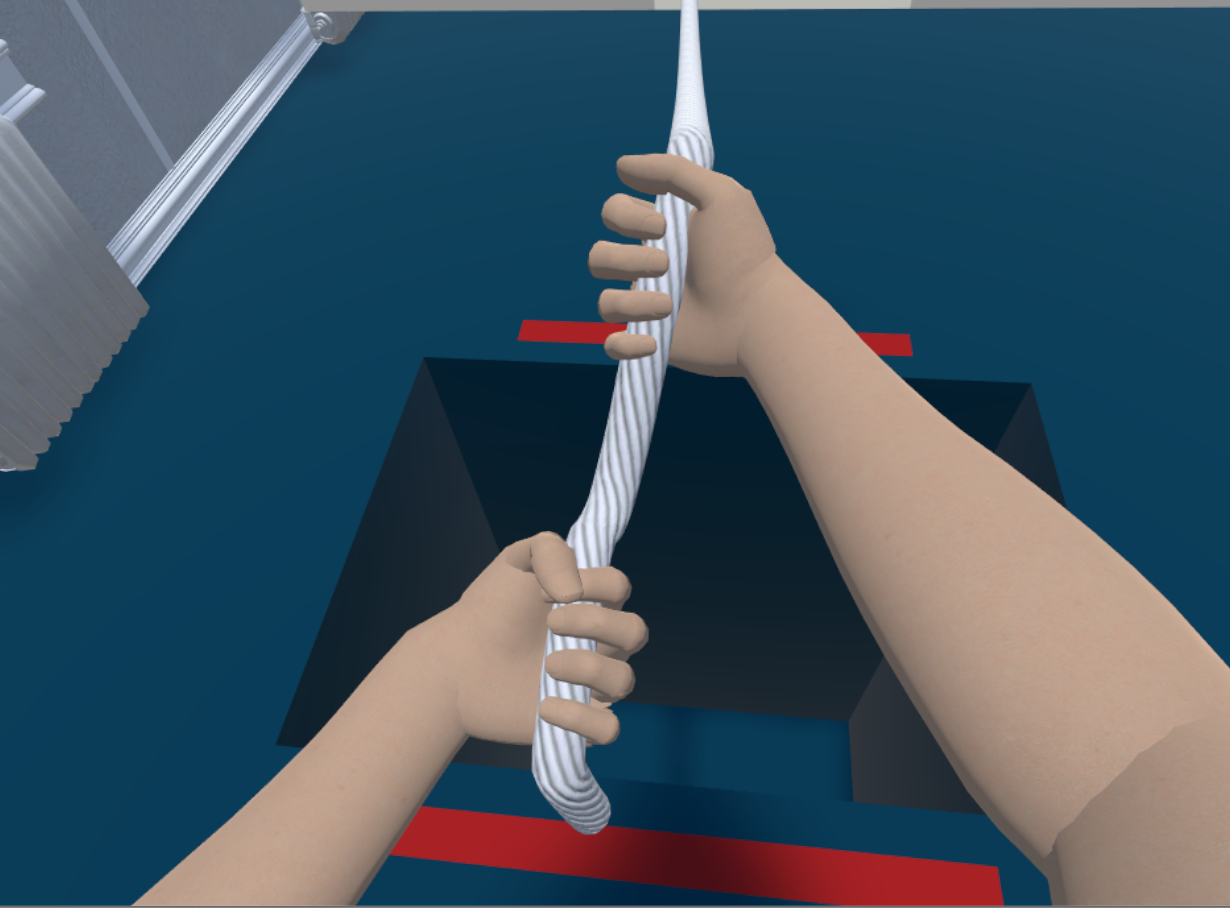
\includegraphics[width=\textwidth]{Images/MaleHand.png}
    \end{minipage}
  \hfill
  \begin{minipage}[b]{0.4\textwidth}
    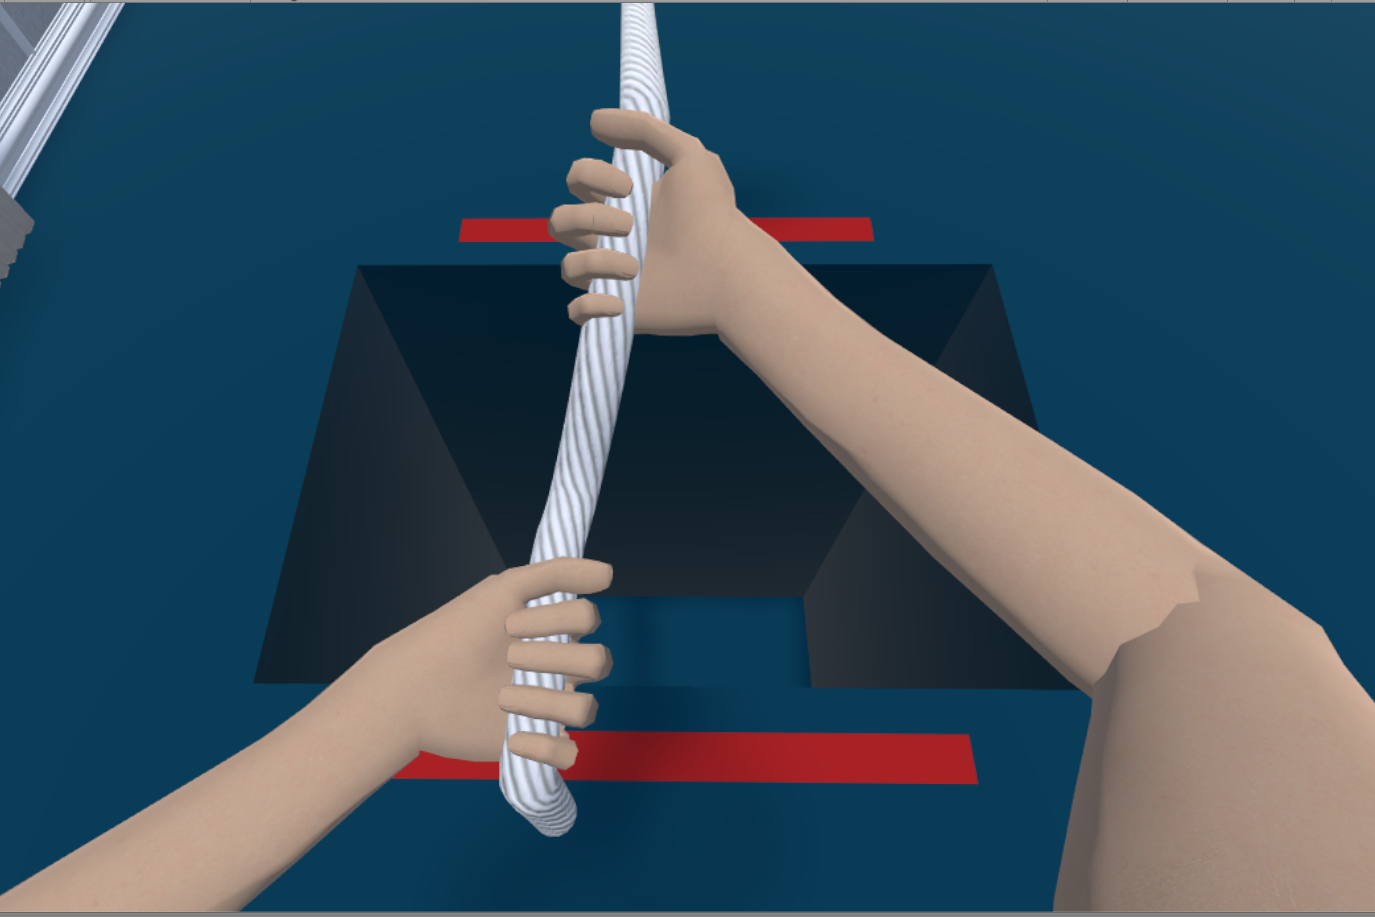
\includegraphics[width=\textwidth]{Images/FemaleHand.png}
      \end{minipage}
\hspace*{\fill}
  \caption{First person view of male (left) and female (right) arms.}
     \label{fig:VRHands}
\end{figure}

In the game players could see their left and right hand holding the rope, which comprised their embodied avatar (seen in figure \ref{fig:VRHands}. The virtual grip of the hands on the rope was taken from a real hand grip of the rope using the HI5 gloves. The finger movement was disabled as the gloves were easily magnetized by the set up and would malfunction shortly after the beginning of the experiment. To prevent loss of ownership from random finger movements, players were told to maintain the same grip on the rope at all times during the experiment. Before starting, users would undergo the calibration of the gloves provided with the HI5 glove set up to maintain accurate hand orientation and position. Despite calibration efforts and manual adjustment trials, the  undesirable finger movement and often inaccurate hand orientation and position proved to be the most difficult set back of this project. This was most challenging when integrating the gloves within an inverse kinematics VR algorithm to display user arm movement in a natural manner.
\\
We used Final IK VR \footnote{https://assetstore.unity.com/packages/tools/animation/final-ik-14290} to display naturalistic avatar body movements. The positions of reference for the algorithm were the left and right hand trackers, together with the headset position. 
This implementations does not always congruently display the position of the virtual arm and user arm. It is, however, an acceptable trade-off in to the lack of elbow tracking and full body tracking. 
The virtual rope was implemented using the Obi Rope asset \footnote{https://assetstore.unity.com/packages/tools/physics/obi-rope-55579}. Its settings were adjusted manually to simulate real rope movements through a trial-and-error approach. Please refer to appendix A for the chosen rope settings. \todo{add rope settings to appendix}. The rope texture was modelled to the real rope users were holding. 

\begin{figure}
  \centering
  \captionsetup{justification=centering,margin=0.1cm}
\hspace*{\fill}
  \begin{minipage}[b]{0.4\textwidth}
    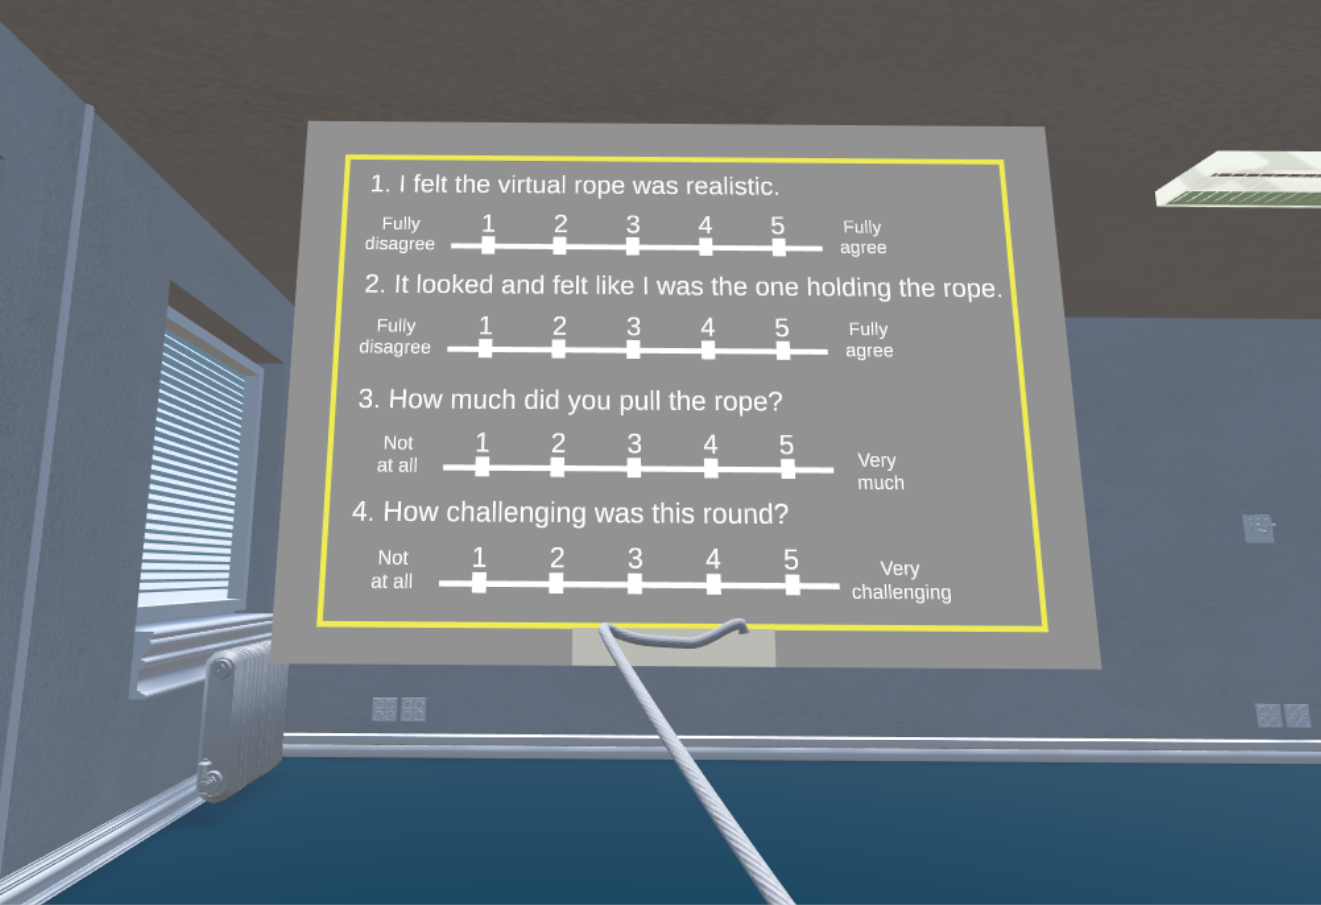
\includegraphics[width=\textwidth]{Images/quizzPanel.png}
    \end{minipage}
  \hfill
  \begin{minipage}[b]{0.4\textwidth}
    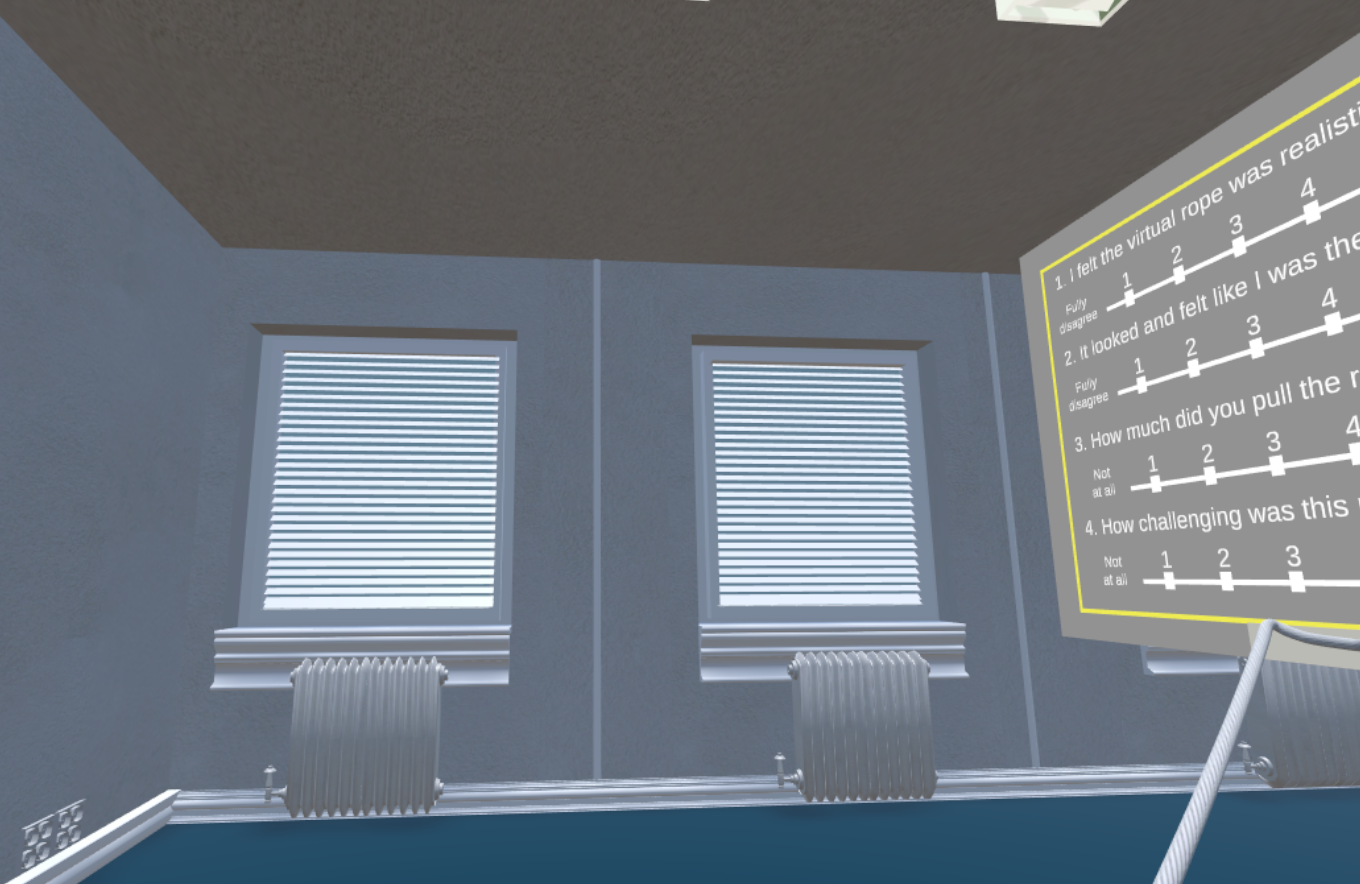
\includegraphics[width=\textwidth]{Images/quizzPanelSide.png}
      \end{minipage}
\hspace*{\fill}
  \caption{Panel with questions in VR, side and left view.}
     \label{fig:VRPanel}
\end{figure}
Between rope-pulls we display a vertical panel with questions \ref{fig:VRPanel}. We used TextMesh Pro\footnote{https://assetstore.unity.com/packages/essentials/beta-projects/textmesh-pro-84126} for the font, to allow for better readability considering the resolution of the headset. Between trials, participants always hold the rope in their hands. In order to still display the rope in users' hands when agents were not holding it, we placed it on the panel as if hanging there. To allow for natural transitions between experiment states, we used a black-out animation lasting one section. This animation fades to black, then fades back into the room scene. During this time, we spawned the questionnaire panel or the opponents. We designed the experiment scene to be as close as possible to the room where the experiment was taking place.
\\
Every second the state of the experiment was logged in a file. Among others, we log users' the gaze target. This was implemented with a Raycast \footnote{https://docs.unity3d.com/ScriptReference/Physics.Raycast.html} originating at the center of the headset. Gaze targets are detected as objects with colliders. Since UMA's and some special parts of the setting (such as the hole) cannot have colliders, we added transparent panels with colliders on top of these objects.
\subsubsection{Agent Design}
\label{section:AgentDesign}

The virtual agents were created in Unity using the Unity Multipurpose Avatar 2 (UMA) asset \footnote{https://assetstore.unity.com/packages/3d/characters/uma-2-unity-multipurpose-avatar-35611} and o3n UMA Races \footnote{https://assetstore.unity.com/packages/3d/characters/humanoids/o3n-male-and-female-uma-races-102187}. We chose this library because the UMA character system has a high degree of avatar customization allowing avatar generation with relative ease. Programmers are able to vary body part sizes such as ear and brow rotations. 
\\
The manipulations described below serve to provide users with a more dynamic experience and make their opponents appear more life-like. We aim to generate high behaviour realism in order to make up for the lack of perceived agency. This serves the purpose of eliciting more realistic responses from people in accordance with the threshold model of social influence \cite{blascovich2002theoretical}. We placed UMAs close enough to participants so they noticed the changes in expression and other animation changes.

\subsubsection{UMA Dna}
We varied perceived strength in the design of the agents and used UMA DNA settings to generate a distribution of agents varying from strong-looking, to average and weak looking. UMA Dna represents a dictionary used to customize Unity multipurpose avatars (UMAs). Appearance can be changed on a scale of 0 to 1, with higher values being used to make adjustments more salient. A downside of this character system is that the magnitudes of these features do not vary linearly and can differ between races and genders. For example, female muscle size cannot be increased on the same scale as male muscle size. Due to this, male agents could have more muscle mass than females. Another example is that increasing lower muscle mass for women inflated the leg muscles in an unnatural way. Furthermore, there were color differences due to mesh materials and textures. 
\\
UMAs in the strong conditions generally had strength-signalling Dna parts closer to 1. Their values decreased to 0.5 for agents in the normal conditions and below 0.5 for agents in the weak condition. We considered the default 0.5 Dna values as average. We manually adjusted these values through trial and error to give UMAs the most human-like appearance and prevent them from looking exceedingly uncanny.    
\subsubsection{Strength Cues}
As strength cues we used muscle tone and fitness, together with adjusted facial proportion as seen in \cite{windhager2011geometric}. Skin, eye and hair color, together with outfit designs were kept as constant as possible between races and genders. For the upper body clothing, the agents had a sleeveless shirt to increase the visibility of the arm muscles. 
With respect to facial manipulations, we varied facial width and jaw size which are known to be associated with testosterone in men \cite{lefevre2013telling}. We decreased the size of the lips and eyes in the strong conditions to increase face-width ratio. While height and age are the best predictors for female perceived strength \cite{sell2008human}, we applied the same variations to the female avatars. We did not adjust height for the agents displayed in the survey images. However, we manipulate height in the user study, increasing height for agents in the strong condition to 0.8 and average to 0.5, keeping avatars in the weak condition at 0.5.  
\\
As strength is closely related to dominance and aggression, we added variables meant to increase intimidation such as tattoos, military hairstyles and manipulated outfit colors. As in previous Proteus effect literature and associated body of work related to social psychology \cite{yee2009proteus,pena2009priming}, we used black clothing to elicit more aggressive attitude perceptions. Agents in the strong conditions had black upper-body clothing, those in medium conditions had gray and for weak agents we used white. While male tattoos are dominantly viewed, female tattoos generate mixed responses from observers \cite{wohlrab2009perception}. As with previous research \cite{van2013proteus}, agents were gender matched to avoid any tensions or similarity biases that would arise from cross-gendered evaluations. Please see section \ref{subsection:thumbnails} for the agents chosen for the surveys.

\subsubsection{Animations}
\label{subsection:animation}
 In addition, we used the UMA Expression Player to even out neutral facial expressions between races and genders. Please refer to appendix X for the neutral expression settings.\todo{ add settings}. The Expression Player was also used at the moment the UMAs were pulling the rope to give the impression that the opponents were exerting themselves or seemed angry. Their facial expressions were exaggerated to be more visible to participants in VR. Additionally, we use the blinking mechanism provided by the UMA Expression Player to make the avatars blink throughout the trials. We interpolate\footnote{https://docs.unity3d.com/ScriptReference/Vector3.Lerp.html} between the changes in facial expression in order to blend them in a natural way.
\\
We used the Mecanim animation system provided by Unity for animation layering and blending. At the start of each trial the opponents are shown with the rope in their hands in an idle posture animation, with their hands moving in the air and their chest moving as if breathing. This animation overlays all other animations and plays throughot the trial. We use the \textit{MORRO MOTION} Idle MoCap for this purpose \footnote{https://assetstore.unity.com/packages/3d/animations/idle-mocap-28345}. After a 3-second countdown, UMAs are triggered with a rope-pulling animation. This animation is derived from the rope pulling animation on Mixamo \footnote{https://www.mixamo.com}.When UMAs reach their maximum-exertion posture, \todo {add pic of avatars pulling} a tugged animation is triggered showing the agents moving their hands back and forth as if the rope was being pulled from them. For the remaining pull time, the UMAs maintain maximum pull posture. This serves the purpose of giving users the impression that their opponents react to the rope being pulled. From the end of the countdown, the rope-pulling lasts 10 seconds. At the beginning of each trial participants have 20 seconds before the countdown starts. This is to allow users to inspect their opponent and look around the room if desired. After the rope pulling ends, there is a 10 second delay before the screen fades the black and the question panel is presented. 
